\documentclass[11pt,a4paper]{article}

\usepackage[utf8]{inputenc}
\usepackage[margin=2.5cm]{geometry}
\usepackage{amsmath,amssymb,amsthm}
\usepackage{booktabs,tabularx,array}
\usepackage{enumitem}
\usepackage{tikz}
\usetikzlibrary{arrows.meta,positioning,patterns}
\usepackage[hidelinks]{hyperref}
\usepackage{xurl}

\newtheorem{proposition}{Proposition}
\newtheorem{lemma}[proposition]{Lemma}
\newtheorem{corollary}[proposition]{Corollary}
\theoremstyle{remark}
\newtheorem{remark}[proposition]{Remark}
\newcommand{\code}[1]{\path{#1}}
\urlstyle{tt}
\newcolumntype{Y}{>{\raggedright\arraybackslash}X}
\newcommand{\sgn}{\operatorname{sign}}
\setlength{\emergencystretch}{3em}

\title{CE375: rational points $(n,x,y)$ on $y^2=(x+6n+3)^2+\dfrac{36n^3+54n^2+27n-58}{x}$\\
via a primitive Booker--Sutherland search\\[2pt]
\large rationale and modus operandi of \texttt{375/gap-search}}
\author{Jamal Agbanwa}
\date{22 November 2026}

\begin{document}
\maketitle

\begin{abstract}
The target is rational $x,y$ with $n$ an integer on
$y^2=(x+6n+3)^2+(36n^3+54n^2+27n-58)/x$, accepting primitive integer points ($\gcd(n,x)=1$, $y$
an integer) and half points ($x=X/2$, $y=Y/2$, $X,Y$ odd, $\gcd(X,Y)=1$). With $A=-x+y$,
$B=-x-y$, $C=2x+6n+3$ the equation is exactly $A^3+B^3+C^3=375$, and the accepted points come from
\emph{primitive} representations of $375=3\cdot5^3$. We show why the existing slope-ordered
(``$d$-first'') engine has a negligible chance of meeting one, and replace it with the
Booker--Sutherland method over $\delta=|a+b|$, restricted by a new primitivity lemma
($5\nmid\delta$ or $125\mid\delta$), with cube roots built for any power of $5$, and aimed at the
frontier of what has already been searched. We compute Heath-Brown's constant for primitive
solutions of 375 from local densities, $\rho_{375}=0.0586$, with the archimedean constant
calibrated on Booker and Sutherland's published values (agreement $0.01\%$). Measured plans for
1{,}800 core-hours give, under the Booker--Sutherland heuristic, a $14\%$, $6\%$ or $2\%$ chance of
a primitive solution if the frontier (largest coordinate already excluded) is $10^{14}$,
$10^{15}$ or $10^{16}$, against about $3\times10^{-10}$ for the slope-ordered engine and $1$ in
$151{,}000$ for $k=114$ on the same hours. The code has 34 tests and an audited pilot.
\end{abstract}

\tableofcontents

%====================================================================
\section{The target and its reduction}\label{sec:reduction}

Put $S=6n+3$ and $N(n)=36n^3+54n^2+27n-58$. Since $S^3=216n^3+324n^2+162n+27$,
\[
  N(n)=\frac{S^3-375}{6}.
\]
The equation is
\begin{equation}\label{eq:E}
  y^2=(x+S)^2+\frac{N(n)}{x},
\end{equation}
and the accepted points are
\begin{enumerate}[leftmargin=*]
  \item \textbf{integer chart:} $n,x,y\in\mathbb Z$ with $\gcd(n,x)=1$;
  \item \textbf{half chart:} $n\in\mathbb Z$, $x=X/2$, $y=Y/2$ with $X,Y$ odd and $\gcd(X,Y)=1$.
\end{enumerate}

\begin{proposition}\label{prop:cubes}
Put $A=-x+y$, $B=-x-y$, $C=2x+S$. Then
\[
  A^3+B^3+C^3-375=-6x\Bigl(y^2-(x+S)^2-\frac{N(n)}{x}\Bigr).
\]
Hence a point of either chart is the same thing as a representation $375=A^3+B^3+C^3$ with
$A+B=-2x\ne0$, and $A,B,C$ are integers in both charts.
\end{proposition}
\begin{proof}
Expand: $A+B=-2x$, $AB=x^2-y^2$, so $A^3+B^3=(A+B)^3-3AB(A+B)=-8x^3+6x(x^2-y^2)$, and
$C^3=(2x+S)^3$. Collecting terms gives $-6x\bigl(y^2-(x+S)^2\bigr)+S^3-375$, and
$S^3-375=6N(n)$. In the half chart $A=(Y-X)/2$, $B=-(X+Y)/2$ and $C=X+S$ are integers because
$X,Y$ are odd.
\end{proof}

Conversely, let $375=a^3+b^3+c^3$. Since $375\equiv6\pmod9$, every component is $\equiv2\pmod3$
(the cubes mod $9$ are $0,\pm1$), and since $375$ is odd, so is $a+b+c$; hence $a+b+c\equiv3\pmod6$
and $n=(a+b+c-3)/6$ is an integer. Each choice of the component $C$ and order $A\ge B$ of the other
two with $A\ne-B$ gives the point $x=-(A+B)/2$, $y=\pm(A-B)/2$: integer chart if $A+B$ is even,
half chart if it is odd.

\paragraph{Primitivity.} A prime dividing $A,B,C$ divides $375$ to the third power, so it is $5$.
A non-primitive representation $5\cdot(a',b',c')$ comes from $3=a'^3+b'^3+c'^3$; for example
$5^3+5^3+5^3=375$ gives $n=2$, $x=-5$, $y=0$, which has $\gcd(n,x)=1$. In the half chart
$\gcd(X,Y)=1$ forces $\gcd(A,B,C)=1$ (a common prime divides $A-B=Y$ and $A+B=-X$). So
\emph{every accepted point comes from a primitive representation}, and the search problem is:
\begin{center}
\emph{find primitive representations $375=a^3+b^3+c^3$, $\gcd(a,b,c)=1$.}
\end{center}
The converter \code{to_points375.py} lists all points of a representation and flags exactly which
are accepted (\code{primitive_point}, \code{primitive_cubes}, \code{desired}), with the same
definitions as the folder \code{375/Scripts for large-scale computations/}.

%====================================================================
\section{Why the slope-ordered engine cannot be expected to succeed}\label{sec:dfirst}

The engine in \code{375/Scripts for large-scale computations/} enumerates slopes
$d=(A+C)/(A+B)=p/q$ in lowest terms by height $H(d)=\max(|p|,q)$ and solves one Thue equation per
slope, for all scalings $g$ up to $10^{100}$. A representation enters through
$A+B=qg$, $A+C=pg$ with $g=\gcd(A+B,A+C)$, so it is reached at height
$\max(|A+B|,|A+C|)/g$. Of the three pair sums one may be small, but at least two are of the size
$M=\max(|a|,|b|,|c|)$; for every labelling the numerator or denominator of $d$ is of size $M$, so
\[
  \text{a representation of size $M$ is reached only if } g\ \ge\ M/H .
\]
Nothing in the problem forces $g$ to be large. For integers of size $M$, $\Pr(g\ge G)\approx
(6/\pi^2)/G$; with six labellings the chance of capture is about $c\,H/M$, $c=36/\pi^2$.
Summing over the Heath-Brown density ($\rho$ solutions per unit $\log M$) beyond a frontier $M_0$,
\[
  E_{\text{slope}}\approx\rho\,c\,H\int_{M_0}^\infty\frac{dM}{M^2}=\frac{\rho\,c\,H}{M_0}.
\]
On 1{,}800 core-hours the engine reaches $H\approx1.5\times10^6$ (its README), which gives
$E_{\text{slope}}/\rho\approx5.5\times10^{-8},\,5.5\times10^{-9},\,5.5\times10^{-10}$ for
$M_0=10^{14},10^{15},10^{16}$. The engine remains the right tool for exact statements about
slopes of small height; it is not a way to find a representation.

%====================================================================
\section{The Booker--Sutherland parametrization}\label{sec:bs}

\begin{lemma}[Booker--Sutherland \cite{BS}]\label{lem:bs}
Let $a^3+b^3+c^3=k$ with $|a|\ge|b|>|c|>\sqrt{|k|}$, and put $\delta=|a+b|$, $z=|c|$,
$\alpha=2^{1/3}-1$. Then $0<\delta<\alpha z$, $z^3\equiv K\pmod\delta$ with $K=k\,\sgn(c)$, and
\[
  \Delta:=\frac{4(z^3-K)/\delta-\delta^2}{3}=(a-b)^2 .
\]
Conversely, if $z^3\equiv K\pmod\delta$ and $\Delta=t^2$ with $t\equiv\delta\pmod2$, then
$s_0=-\sgn(c)\delta$, $a=(s_0+t)/2$, $b=(s_0-t)/2$ give a solution.
\end{lemma}

For $k\equiv6\pmod9$ (as for 114), all components are $\equiv2\pmod 3$, so $3\nmid\delta$,
$z\equiv\delta\pmod3$, $9\mid\Delta$, and $\Delta\equiv1\pmod8$ for odd $\delta$; these fix $z$ to a
few classes modulo $9\delta$ (or $18\delta$), exactly as in the $k=114$ engine \cite{CE114}.

\subsection{A primitivity lemma}
\begin{lemma}\label{lem:prim}
Let $p\ne3$ be a prime with $p^3\mid k$ and $p\equiv2\pmod3$. If $a^3+b^3+c^3=k$ with
$\gcd(a,b,c)=1$ and $\delta=|a+b|\ne0$, then $v_p(\delta)=0$ or $v_p(\delta)\ge3$.
\end{lemma}
\begin{proof}
If $p\nmid c$, then $a^3+b^3=k-c^3\not\equiv0\pmod p$, so $p\nmid a+b$. If $p\mid c$, then $p\nmid a$:
otherwise $p\mid b^3=k-a^3-c^3$ and $p\mid\gcd(a,b,c)$; likewise $p\nmid b$. If $p\mid a+b$ then
$a\equiv-b$ and $a^2-ab+b^2\equiv3b^2\not\equiv0\pmod p$, so
$v_p(a+b)=v_p(a^3+b^3)=v_p(k-c^3)\ge\min(v_p(k),3v_p(c))\ge3$.
\end{proof}

For $375$ ($p=5$) the $\delta$ with $5\parallel\delta$ or $25\parallel\delta$ cannot carry a
primitive solution: $19.2\%$ of the $\delta$ prime to $3$ are skipped (\texttt{--primitive}).
Every $\delta$ prime to $5$ carries only primitive solutions; for $125\mid\delta$ each hit is
tagged with $\gcd(a,b,c)$. The hypothesis $p\equiv2\pmod3$ is needed: for $p\equiv1\pmod3$,
$a^3\equiv-b^3$ allows $a\equiv-\zeta b$ with $\zeta$ a cube root of unity, and the worker refuses
such $k$ in primitive mode.

\subsection{Cube roots modulo prime powers dividing $k$}
Write $k=p^vu$ with $p\nmid u$, $p\ne3$. The roots of $z^3\equiv k\pmod{p^e}$ are:
\begin{itemize}[leftmargin=*]
  \item for $e\le v$: the multiples of $p^{\lceil e/3\rceil}$ ($p^{e-\lceil e/3\rceil}$ roots);
  \item for $e>v$: none unless $3\mid v$; then $z=p^{v/3}z'$ with $z'^3\equiv u\pmod{p^{e-v}}$, and $z'$
  free modulo $p^{e-v/3}$.
\end{itemize}
For $375$ there are $25$ roots modulo $5^e$ for every $e\ge3$. The worker constructs them (cube
roots modulo $p$, Hensel lifting, then the $p^{2v/3}$ free digits); the inherited code enumerated
$z$ modulo $p^e$ and refused $5^{11}\mid\delta$.

%====================================================================
\section{The frontier and the yield model}\label{sec:model}

\subsection{What has been searched}
Booker and Sutherland's large searches \cite{BS,Booker} use an algorithm stated for cube-free
$k$ \cite{Suth22}, so $375$ may not have been included. The searches that cover all $k<1000$,
primitive solutions of $375$ included, are Elkies-type searches by largest coordinate:
Elsenhans--Jahnel to $10^{14}$ \cite{EJ}, Huisman to $10^{15}$ \cite{Huisman}. We call the
largest coordinate $N$ below which primitive solutions are excluded the \emph{frontier}; it is a
parameter of the planner (\texttt{--frontier}, default $10^{14}$) and must be confirmed before a
campaign (Section~\ref{sec:limits}).

\subsection{The frontier in the $(\delta,z)$ plane}
By Lemma~\ref{lem:bs} the largest coordinate is $(\delta+t)/2$ with $t=\sqrt\Delta$. It exceeds
$N$ exactly when $\Delta>(2N-\delta)^2$, i.e.\ ($k$ negligible)
\begin{equation}\label{eq:frontier}
  z^3>z_N(\delta)^3:=\frac{\delta\bigl(3(2N-\delta)^2+\delta^2\bigr)}{4}\ \approx\ 3\delta N^2 .
\end{equation}
So the unsearched region lies above a curve of slope $1/3$ in $(\log\delta,\log z)$, and it
reaches down to small $\delta$ for large $z/\delta$ (Figure~\ref{fig:plane}).

\begin{figure}[ht]
\centering
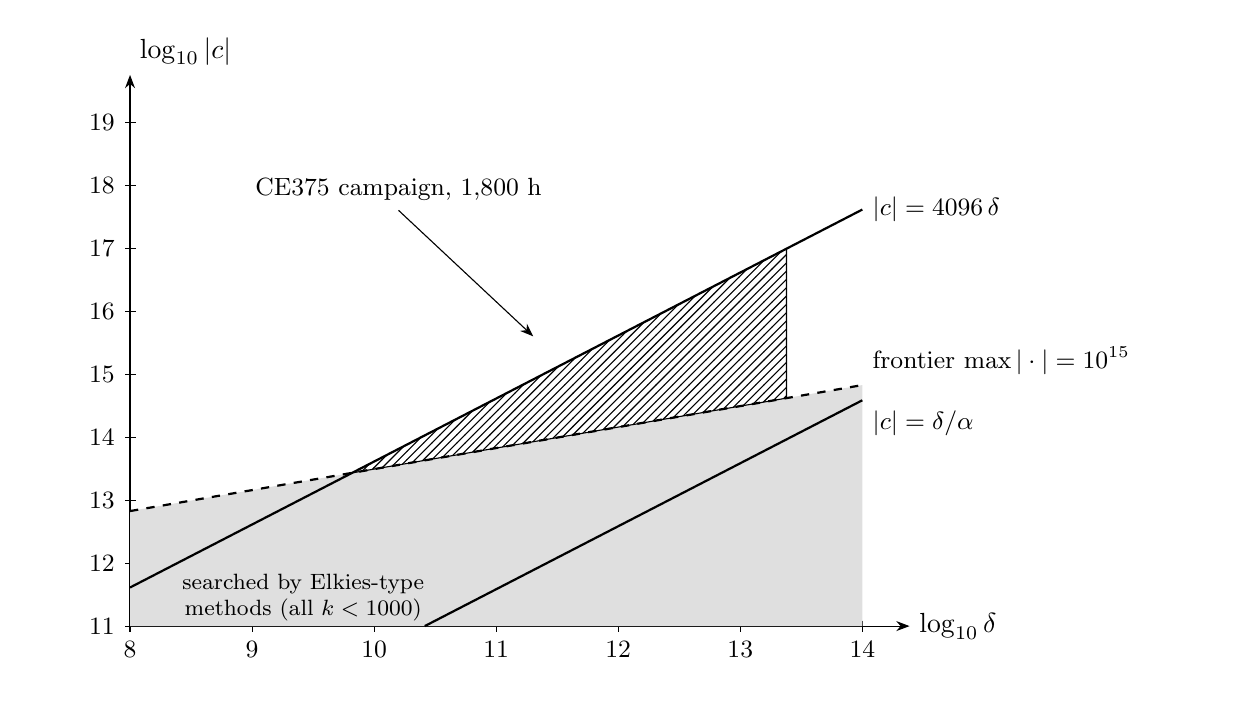
\begin{tikzpicture}
  \clip (-1.3,-0.7) rectangle (13.8,7.6);
  \draw[-{Stealth}] (0,0) -- (9.9,0) node[right]{$\log_{10}\delta$};
  \draw[-{Stealth}] (0,0) -- (0,7.0) node[above right]{$\log_{10}|c|$};
  \draw (0.00,0.07)--(0.00,-0.07) node[below]{\small 8};
  \draw (1.55,0.07)--(1.55,-0.07) node[below]{\small 9};
  \draw (3.10,0.07)--(3.10,-0.07) node[below]{\small 10};
  \draw (4.65,0.07)--(4.65,-0.07) node[below]{\small 11};
  \draw (6.20,0.07)--(6.20,-0.07) node[below]{\small 12};
  \draw (7.75,0.07)--(7.75,-0.07) node[below]{\small 13};
  \draw (9.30,0.07)--(9.30,-0.07) node[below]{\small 14};
  \draw (0.07,0.00)--(-0.07,0.00) node[left]{\small 11};
  \draw (0.07,0.80)--(-0.07,0.80) node[left]{\small 12};
  \draw (0.07,1.60)--(-0.07,1.60) node[left]{\small 13};
  \draw (0.07,2.40)--(-0.07,2.40) node[left]{\small 14};
  \draw (0.07,3.20)--(-0.07,3.20) node[left]{\small 15};
  \draw (0.07,4.00)--(-0.07,4.00) node[left]{\small 16};
  \draw (0.07,4.80)--(-0.07,4.80) node[left]{\small 17};
  \draw (0.07,5.60)--(-0.07,5.60) node[left]{\small 18};
  \draw (0.07,6.40)--(-0.07,6.40) node[left]{\small 19};
  \fill[gray!25] (0,0) -- (0.000,1.461) -- (0.310,1.514) -- (0.620,1.567) -- (0.930,1.621) -- (1.240,1.674) -- (1.550,1.727) -- (1.860,1.781) -- (2.170,1.834) -- (2.480,1.887) -- (2.790,1.941) -- (3.100,1.994) -- (3.410,2.047) -- (3.720,2.101) -- (4.030,2.154) -- (4.340,2.207) -- (4.650,2.261) -- (4.960,2.314) -- (5.270,2.367) -- (5.580,2.421) -- (5.890,2.474) -- (6.200,2.527) -- (6.510,2.581) -- (6.820,2.634) -- (7.130,2.687) -- (7.440,2.741) -- (7.750,2.794) -- (8.060,2.847) -- (8.370,2.901) -- (8.680,2.954) -- (8.990,3.007) -- (9.300,3.061) -- (9.300,0) -- cycle;
  \draw[thick,dashed] (0.000,1.461) -- (0.310,1.514) -- (0.620,1.567) -- (0.930,1.621) -- (1.240,1.674) -- (1.550,1.727) -- (1.860,1.781) -- (2.170,1.834) -- (2.480,1.887) -- (2.790,1.941) -- (3.100,1.994) -- (3.410,2.047) -- (3.720,2.101) -- (4.030,2.154) -- (4.340,2.207) -- (4.650,2.261) -- (4.960,2.314) -- (5.270,2.367) -- (5.580,2.421) -- (5.890,2.474) -- (6.200,2.527) -- (6.510,2.581) -- (6.820,2.634) -- (7.130,2.687) -- (7.440,2.741) -- (7.750,2.794) -- (8.060,2.847) -- (8.370,2.901) -- (8.680,2.954) -- (8.990,3.007) -- (9.300,3.061) node[above right,font=\small,align=left]{frontier $\max|\cdot|=10^{15}$};
  \draw[thick] (3.743,0.000) -- (9.300,2.868) node[below right,font=\small]{$|c|=\delta/\alpha$};
  \draw[thick] (0.000,0.490) -- (9.300,5.290) node[right,font=\small]{$|c|=4096\,\delta$};
  \fill[pattern=north east lines] (2.853,1.951) -- (2.994,1.976) -- (3.134,2.000) -- (3.275,2.024) -- (3.416,2.048) -- (3.556,2.072) -- (3.697,2.097) -- (3.837,2.121) -- (3.978,2.145) -- (4.119,2.169) -- (4.259,2.193) -- (4.400,2.218) -- (4.540,2.242) -- (4.681,2.266) -- (4.822,2.290) -- (4.962,2.314) -- (5.103,2.338) -- (5.243,2.363) -- (5.384,2.387) -- (5.525,2.411) -- (5.665,2.435) -- (5.806,2.459) -- (5.947,2.484) -- (6.087,2.508) -- (6.228,2.532) -- (6.368,2.556) -- (6.509,2.580) -- (6.650,2.605) -- (6.790,2.629) -- (6.931,2.653) -- (7.071,2.677) -- (7.212,2.701) -- (7.353,2.726) -- (7.493,2.750) -- (7.634,2.774) -- (7.774,2.798) -- (7.915,2.822) -- (8.056,2.846) -- (8.196,2.871) -- (8.337,2.895) -- (8.337,4.793) -- (8.196,4.720) -- (8.056,4.647) -- (7.915,4.575) -- (7.774,4.502) -- (7.634,4.430) -- (7.493,4.357) -- (7.353,4.285) -- (7.212,4.212) -- (7.071,4.139) -- (6.931,4.067) -- (6.790,3.994) -- (6.650,3.922) -- (6.509,3.849) -- (6.368,3.777) -- (6.228,3.704) -- (6.087,3.631) -- (5.947,3.559) -- (5.806,3.486) -- (5.665,3.414) -- (5.525,3.341) -- (5.384,3.268) -- (5.243,3.196) -- (5.103,3.123) -- (4.962,3.051) -- (4.822,2.978) -- (4.681,2.906) -- (4.540,2.833) -- (4.400,2.760) -- (4.259,2.688) -- (4.119,2.615) -- (3.978,2.543) -- (3.837,2.470) -- (3.697,2.398) -- (3.556,2.325) -- (3.416,2.252) -- (3.275,2.180) -- (3.134,2.107) -- (2.994,2.035) -- (2.853,1.962) -- cycle;
  \draw (2.853,1.951) -- (2.994,1.976) -- (3.134,2.000) -- (3.275,2.024) -- (3.416,2.048) -- (3.556,2.072) -- (3.697,2.097) -- (3.837,2.121) -- (3.978,2.145) -- (4.119,2.169) -- (4.259,2.193) -- (4.400,2.218) -- (4.540,2.242) -- (4.681,2.266) -- (4.822,2.290) -- (4.962,2.314) -- (5.103,2.338) -- (5.243,2.363) -- (5.384,2.387) -- (5.525,2.411) -- (5.665,2.435) -- (5.806,2.459) -- (5.947,2.484) -- (6.087,2.508) -- (6.228,2.532) -- (6.368,2.556) -- (6.509,2.580) -- (6.650,2.605) -- (6.790,2.629) -- (6.931,2.653) -- (7.071,2.677) -- (7.212,2.701) -- (7.353,2.726) -- (7.493,2.750) -- (7.634,2.774) -- (7.774,2.798) -- (7.915,2.822) -- (8.056,2.846) -- (8.196,2.871) -- (8.337,2.895) -- (8.337,4.793) -- (8.196,4.720) -- (8.056,4.647) -- (7.915,4.575) -- (7.774,4.502) -- (7.634,4.430) -- (7.493,4.357) -- (7.353,4.285) -- (7.212,4.212) -- (7.071,4.139) -- (6.931,4.067) -- (6.790,3.994) -- (6.650,3.922) -- (6.509,3.849) -- (6.368,3.777) -- (6.228,3.704) -- (6.087,3.631) -- (5.947,3.559) -- (5.806,3.486) -- (5.665,3.414) -- (5.525,3.341) -- (5.384,3.268) -- (5.243,3.196) -- (5.103,3.123) -- (4.962,3.051) -- (4.822,2.978) -- (4.681,2.906) -- (4.540,2.833) -- (4.400,2.760) -- (4.259,2.688) -- (4.119,2.615) -- (3.978,2.543) -- (3.837,2.470) -- (3.697,2.398) -- (3.556,2.325) -- (3.416,2.252) -- (3.275,2.180) -- (3.134,2.107) -- (2.994,2.035) -- (2.853,1.962) -- cycle;
  \node[font=\footnotesize,align=center] at (2.2,0.36) {searched by Elkies-type\\methods (all $k<1000$)};
  \draw[-{Stealth}] (3.41,5.28) node[above,font=\small]{CE375 campaign, 1{,}800 h} -- (5.12,3.68);
\end{tikzpicture}

\caption{The $(\log\delta,\log|c|)$ plane for primitive solutions of $375$. Solutions satisfy
$|c|>\delta/\alpha$. Grey: below the frontier \eqref{eq:frontier} for $N=10^{15}$. Hatched: the
1{,}800-hour campaign of Section~\ref{sec:plans} ($\delta\in[5.6\cdot10^9,2.4\cdot10^{13})$,
$|c|\le4096\,\delta$); only its part above the frontier carries new weight.}
\label{fig:plane}
\end{figure}

\subsection{The density model}
Booker and Sutherland model the solutions with a given $\delta$ as having $|c|/\delta$ distributed
with tail $cK(R)\sim(\alpha R)^{-1/2}$; normalised by Heath-Brown's conjecture \cite{HB} that the
number of solutions of height at most $B$ is $\rho\log B$, this is the density
\[
  dE=\frac{\rho}{2\sqrt\alpha}\,\delta^{-1/2}z^{-3/2}\,d\delta\,dz\qquad(z>\delta/\alpha).
\]
The expected number of primitive solutions in a campaign $\delta\in[D_0,D_1)$, $z\le R\delta$,
beyond the frontier is therefore
\begin{equation}\label{eq:yield}
  E=\rho\int_{D_0}^{D_1}\frac{\ell(\delta)^{-1/2}-(R\delta)^{-1/2}}{\sqrt{\alpha\,\delta}}\,d\delta,
  \qquad \ell(\delta)=\max\bigl(\delta/\alpha,\ z_N(\delta)\bigr),
\end{equation}
with the integrand set to $0$ where $\ell(\delta)\ge R\delta$. Without a frontier this is
$\rho\,(1-1/\sqrt{\alpha R})\ln(D_1/D_0)$, the formula used for $k=114$. The planner integrates
\eqref{eq:yield} numerically in $\log\delta$.

%====================================================================
\section{Heath-Brown's constant for primitive solutions of 375}\label{sec:rho}

Booker and Sutherland tabulate $\rho$ only for cube-free $k$. We compute it from local densities,
\[
  \rho_k=C\prod_p\sigma_p(k),\qquad \sigma_p(k)=\lim_{e\to\infty}\frac{N^*_k(p^e)}{p^{2e}},
\]
where $N^*_k(p^e)$ counts solutions modulo $p^e$ that are not all divisible by $p$ (the primitive
solutions; for cube-free $k$ this restriction is empty). The archimedean factor $C$ does not depend
on $k$, because the $\log B$ growth of the real density comes from the cone $x^3+y^3+z^3=0$.

\begin{proposition}\label{prop:np}
Let $p\equiv1\pmod3$, $p\nmid3k$, and write $4p=L^2+27M^2$ with $L\equiv1\pmod3$. Then the number of
solutions of $x^3+y^3+z^3\equiv k\pmod p$ is
\[
  N_p(k)=\begin{cases}p^2+6p-L&\text{if $k$ is a cube mod $p$},\\ p^2-3p-L&\text{otherwise.}\end{cases}
\]
For $p\equiv2\pmod3$, $p\nmid3k$, $N_p(k)=p^2$. In both cases $\sigma_p=N_p/p^2$.
\end{proposition}
\begin{proof}
With $\chi$ a cubic character, $N_p(k)=p^2+\sum_{\chi_i\in\{\chi,\bar\chi\}}(\chi_1\chi_2\chi_3)(k)\,
J(\chi_1,\chi_2,\chi_3)$ \cite[Ch.~8, \S7]{IR}. The six terms with two equal characters have
$J=g(\chi)g(\bar\chi)=p$ and contribute $3p(\chi(k)+\bar\chi(k))$; the terms $(\chi,\chi,\chi)$ and
$(\bar\chi,\bar\chi,\bar\chi)$ have trivial product and $J=-J(\chi,\chi)$, resp.\ its conjugate.
With $J(\chi,\chi)=a+b\omega$, $a\equiv-1$, $b\equiv0\pmod3$, one has $2\operatorname{Re}J=2a-b=L$.
For $p\equiv2\pmod3$ cubing is a bijection. The surface is smooth modulo $p\nmid3k$, so Hensel's lemma
gives $\sigma_p=N_p/p^2$. The formula is also checked by brute force for every $k\bmod p$,
$p\le67$ (\code{tests/test_rho.py}).
\end{proof}

For $p\mid3k$ the densities are counted exactly modulo $p^e$ until they are constant in $e$:

\begin{center}
\begin{tabular}{lll}
\toprule
$k$ & factors at $p\mid3k$ & note\\
\midrule
114 & $\sigma_2=0.75$, $\sigma_3=1/3$, $\sigma_{19}=1.346260$ & cube-free\\
390 & $\sigma_2=0.75$, $\sigma_3=1/3$, $\sigma_5=0.96$, $\sigma_{13}=0.639053$ & cube-free\\
627 & $\sigma_3=1/3$, $\sigma_{11}=0.991736$, $\sigma_{19}=1.346260$ & cube-free\\
375 & $\sigma_3=1/3$, $\sigma_5=0.96=24/25$ & primitive solutions only\\
\bottomrule
\end{tabular}
\end{center}

\noindent (Counting all solutions of 375, primitive or not, would change $\sigma_5$; the test suite
checks that.) The product over $p\equiv1\pmod3$ is an Euler product for a cubic Hecke $L$-function at
$s=1$ and converges only conditionally, so it is truncated at $P$ and the convergence displayed:

\begin{center}
\begin{tabular}{rcccc}
\toprule
$P$ & $\prod_{p\le P}\sigma_p$ (all local factors), 114 & 390 & 627 & 375\\
\midrule
$10^5$ & 0.099123 & 0.055832 & 0.220162 & 0.099604\\
$10^6$ & 0.099332 & 0.055916 & 0.220111 & 0.099553\\
$10^7$ & 0.099278 & 0.055929 & 0.220074 & 0.099540\\
$10^8$ & 0.099282 & 0.055929 & 0.220020 & 0.099530\\
\bottomrule
\end{tabular}
\end{center}

\noindent Calibrating $C=\rho^{\rm BS}_k/\prod\sigma_p$ on Booker and Sutherland's Table~1
($\rho_{114}=0.058459$, $\rho_{390}=0.032935$, $\rho_{627}=0.129565$) at $P=10^8$ gives
\[
  C=0.588818,\ 0.588868,\ 0.588879\qquad(\text{spread }0.01\%),
\]
which checks the local factors, the formula of Proposition~\ref{prop:np} and the claim that $C$ is
independent of $k$ at once. With the mean $C=0.588855$:
\[
  \rho_{375}^{\rm prim}=0.05865,\ 0.05862,\ 0.05862,\ 0.05861\qquad(P=10^5,\dots,10^8),
\]
so $\boxed{\rho_{375}=0.0586}$, within $\pm0.0001$; almost exactly $\rho_{114}=0.05846$. The
computation is \code{tools/rho.py} (about ten seconds) and its output is
\code{validation/rho-P1e8.txt}.

%====================================================================
\section{The engine}\label{sec:engine}

The worker \code{src/gap_worker.cpp} (version 1.2.0) is the $k=114$ worker 1.1.0 \cite{CE114} with
the changes of Section~\ref{sec:bs}. For each $\delta$ in a task it
\begin{enumerate}[leftmargin=*]
  \item factors $\delta$ with a segmented sieve, rejecting $\delta$ with a prime $p\equiv1\pmod3$
  modulo which $375$ is not a cube (equivalently $3$ is not, $p\ne5$);
  \item skips $3\mid\delta$ and, with \texttt{--primitive}, $v_5(\delta)\in\{1,2\}$; this test is
  made on $\delta$ itself, so the counters do not depend on how a range is split (the audit's
  precondition; a regression test enforces it);
  \item computes all cube roots of $\pm375$ modulo $\delta$ (Section~\ref{sec:bs}, CRT);
  \item walks $z$ in the classes modulo $9\delta$ or $18\delta$ over
  $\lfloor3.847\delta\rfloor\le z\le R\delta$, with 128-bit $z$ and a bit-parallel filter of 16
  exact quadratic-residue conditions on $\Delta$;
  \item decides survivors exactly with GMP, verifies $a^3+b^3+c^3=375$ and prints the hit with
  \texttt{"primitive"}$=[\gcd(a,b,c)=1]$.
\end{enumerate}
The filters are necessary conditions, so nothing in the searched region is lost. The pipeline
(\code{gap_campaign.py}, \code{run_gap_task.py}, \code{collect_gap.py}, \code{audit_gap.py}) is
that of the $k=114$ campaign, with the primitive flag carried through tasks, checkpoints, collection
and audit, and \code{to_points375.py} turning hits into points of \eqref{eq:E}.

%====================================================================
\section{Measured plans for 1{,}800 core-hours}\label{sec:plans}

Cost per $\delta$ (\code{gap_campaign.py} \texttt{--calibrate}, $k=375$, \texttt{--primitive}, one core of
the development host):

\begin{center}
\begin{tabular}{rrr}
\toprule
$R$ & $\mu$s per $\delta$ at $\delta=10^{10}$ & at $\delta=10^{12}$\\
\midrule
1024 & 0.211 & 0.221\\
2048 & 0.245 & 0.238\\
4096 & 0.271 & 0.289\\
8192 & 0.385 & 0.367\\
16384 & 0.463 & 0.553\\
32768 & 0.700 & 0.690\\
65536 & 1.206 & 1.186\\
\bottomrule
\end{tabular}
\end{center}

\noindent \code{gap_campaign.py} \texttt{--optimize} maximises \eqref{eq:yield} over the starting $\delta$
and $R$ for the budget. With $\rho_{375}=0.0586$:

\begin{center}
\begin{tabularx}{\linewidth}{lYrrrr}
\toprule
frontier $N$ & plan & $E/\rho$ & $E$ & $\Pr(\ge1)$ & $E$, slope-ordered\\
\midrule
$10^{14}$ & $\delta\in[5.6\cdot10^8,2.4\cdot10^{13})$, $R=4096$ & 2.66 & 0.156 & \textbf{14.4\%} & $3\cdot10^{-9}$\\
$10^{15}$ & $\delta\in[5.6\cdot10^9,2.4\cdot10^{13})$, $R=4096$ & 1.07 & 0.063 & \textbf{6.1\%} & $3\cdot10^{-10}$\\
$10^{16}$ & $\delta\in[5.6\cdot10^9,1.4\cdot10^{13})$, $R=16384$ & 0.39 & 0.023 & \textbf{2.3\%} & $3\cdot10^{-11}$\\
\bottomrule
\end{tabularx}
\end{center}

\noindent For comparison, the $k=114$ campaign on the same hours has $E=6.6\times10^{-6}$ (1 in
151{,}000): for $114$ the unsearched region starts at $\delta=1.85\times10^{17}$, where each
$\delta$ carries far less weight. More hours raise $E$ roughly logarithmically, as $\delta$ moves
past the frontier curve.

%====================================================================
\section{Validation}\label{sec:validation}

\texttt{make test} runs 34 tests.
\begin{itemize}[leftmargin=*]
\item \textbf{Inherited engine tests (16):} the record solutions for $k=33,42,3,165,579,795,906$; a
brute force for every $k\equiv\pm3\pmod9$ up to $100$; filter verdicts against exact arithmetic,
including $z\ge2^{64}$; factorizations and roots at production size; the plan--run--interrupt--%
resume--collect cycle; coverage accounting and the audit.
\item \textbf{Cube factors and primitivity (15):}
  \begin{itemize}
  \item roots modulo every $\delta<2500$ against brute force for $k=24,375,1875,3000,7125,-375$,
  and root counts at $\delta\approx10^{13}$ divisible by $5^e$, $e\le17$;
  \item Lemma~\ref{lem:prim} on every primitive solution with coordinates up to $600$ for those $k$;
  \item a brute force over coordinates up to $1500$ for $k=24,48,375,750,1875,3000,6000,7125$:
  without \texttt{--primitive} exactly the solutions in the region with correct flags, with it
  exactly the primitive ones;
  \item identical hits with the filters disabled; $5\times$(the $k=3$ record) found and tagged
  non-primitive without \texttt{--primitive} and skipped with it; cube-free $k$ unaffected;
  $k=3\cdot7^3$ refused;
  \item counters independent of how a range is split;
  \item the converter against \code{common375.py} of the slope-ordered folder (points and flags);
  \item the yield model: closed form without a frontier, frontier placed exactly;
  \item an end-to-end campaign at $k=7125=57\cdot5^3$ that finds its primitive solution
  $(-67)^3+(-46)^3+74^3$, collects it as primitive, audits cleanly and converts it to two
  accepted half-chart points.
  \end{itemize}
\item \textbf{$\rho$ (3):} Proposition~\ref{prop:np} against brute force; the exact local factors
$\sigma_3=1/3$, $\sigma_5=24/25$; the calibration constant equal for 114, 390, 627 to $0.5\%$ at
$P=10^6$ with $\rho_{375}\in[0.0580,0.0592]$.
\end{itemize}

\paragraph{Pilot at $k=375$.} Worker 1.2.0, 22 November 2026, through plan, run, collect and a
$5\%$ audit; $\delta\in[5623413252,7623413252)$, $R=4096$, \texttt{--primitive}, two tasks in
parallel on the two-core development host.

\begin{center}
\begin{tabular}{lr}
\toprule
$\delta$ values (gaps: none) & 2{,}000{,}000{,}000\\
skipped: $3\mid\delta$ / Lemma~\ref{lem:prim} / no cube root & 666{,}666{,}667 / 256{,}000{,}000 / 700{,}605{,}724\\
$\delta$ processed, cube roots & 376{,}727{,}609, 953{,}402{,}561\\
candidates $z$ & 325{,}122{,}046{,}498\\
exact GMP checks & 9{,}953{,}920\\
worker time & 0.154 core-hours (0.28\,$\mu$s per $\delta$)\\
audit & 6/6 chunks reproduce exactly\\
representations of 375 & 0\\
\bottomrule
\end{tabular}
\end{center}

\noindent The first audit of an earlier build disagreed on the split between the primitivity skip
and ``no cube root'', because the skip was read from sieve factor lists that depend on the sieve
limit, hence on a task's $\delta_{\rm stop}$. It now reads $\delta$ itself, and a regression test
requires identical counters however a range is split.

%====================================================================
\section{What a run proves, and what must be checked first}\label{sec:limits}

A completed, collected and audited campaign proves that $375$ has \emph{no} primitive
representation with $\delta=|a+b|$ in the covered range and $3.847\,\delta\le|c|\le R\delta$, hence
no accepted point $(n,x,\pm y)$ of either chart arising from one. This statement does not depend on
any heuristic.

The probabilities of Section~\ref{sec:plans} rest on Heath-Brown's conjecture, on the
Booker--Sutherland model (formulated for cube-free $k$; we assume the same distribution in
$(\delta,z)$ for primitive solutions of $375$, the $5$-adic structure being accounted for in
$\rho$), and on the frontier. Before committing the hours:
\begin{enumerate}[leftmargin=*]
  \item \textbf{Confirm the frontier.} Ask Booker or Sutherland (or Charity Engine) whether a search
  beyond the Elkies-type bounds has covered primitive solutions of $375$. A higher frontier lowers
  the odds as in the table; a search that covered this $(\delta,z)$ region would make the campaign
  redundant.
  \item \textbf{Calibrate on the grid's CPU} and re-run \texttt{--optimize}: the best $R$ and starting
  $\delta$ depend on the measured cost.
\end{enumerate}

%====================================================================
\appendix
\section{Files}
\begin{center}
\begin{tabularx}{\linewidth}{lY}
\toprule
file (in \code{375/gap-search/}) & role\\
\midrule
\code{src/gap_worker.cpp} & the engine, version 1.2.0 (Section~\ref{sec:engine})\\
\code{gap_common.py} & task validation, exact hit verification, primitivity rule, yield model, $\rho$\\
\code{gap_campaign.py} & calibration, \texttt{--optimize}, budget sizing, tasks and \code{page.json}\\
\code{run_gap_task.py}, \code{collect_gap.py}, \code{audit_gap.py} & runner with checkpoints, collection with gap report, audit\\
\code{to_points375.py} & representation $\to$ points $(n,x,\pm y)$ with flags, verified on \eqref{eq:E}\\
\code{tools/rho.py} & the computation of Section~\ref{sec:rho}\\
\code{tests/} & \code{test_engine.py} (16), \code{test_375.py} (15), \code{test_rho.py} (3)\\
\code{validation/rho-P1e8.txt} & output of \code{tools/rho.py --P 1e8}\\
\code{README.md} & operating guide\\
\code{Dockerfile}, \code{container_entrypoint.sh} & Charity Engine image (tests run at build)\\
\bottomrule
\end{tabularx}
\end{center}

\begin{thebibliography}{9}
\bibitem{BS} A.~R. Booker and A.~V. Sutherland, \emph{On a question of Mordell}, Proc.\ Natl.\ Acad.\
Sci.\ USA \textbf{118} (2021), e2022377118; arXiv:2007.01209.
\bibitem{Booker} A.~R. Booker, \emph{Cracking the problem with 33}, Res.\ Number Theory \textbf{5}
(2019), 26.
\bibitem{CE114} J.~Agbanwa, \emph{CE114: rational $d$ via the Booker--Sutherland gap search},
\code{114 /Algorithm for computation /ce114_rationale.pdf}, November 2026.
\bibitem{EJ} A.-S. Elsenhans and J.~Jahnel, \emph{New sums of three cubes}, Math.\ Comp.\ \textbf{78}
(2009), 1227--1230.
\bibitem{Elkies} N.~D. Elkies, \emph{Rational points near curves and small nonzero $|x^3-y^2|$ via
lattice reduction}, ANTS IV (2000); arXiv:math/0005139.
\bibitem{HB} D.~R. Heath-Brown, \emph{The density of zeros of forms for which weak approximation
fails}, Math.\ Comp.\ \textbf{59} (1992), 613--623.
\bibitem{Huisman} S.~G. Huisman, \emph{Newer sums of three cubes}, arXiv:1604.07746 (2016).
\bibitem{IR} K.~Ireland and M.~Rosen, \emph{A Classical Introduction to Modern Number Theory}, 2nd
ed., Springer, 1990, Chapter~8.
\bibitem{Suth22} A.~V. Sutherland, \emph{Sums of three cubes} (Mordell's question), lecture
slides, 2022, \url{https://math.mit.edu/~drew/Mordell2022.pdf}.
\end{thebibliography}

\end{document}
